\section{Introduction}\label{sec:intro}
In many real-world settings, the passage of large vehicles or transport units is
obstructed by movable obstacles such as pallets, boxes, or equipment, motivating
the deployment of mobile robot teams to actively clear traversable corridors and
enable safe passage. This capability is particularly critical in cluttered and
unstructured environments—warehouses, disaster sites, and dense urban spaces—
where conventional path planning methods assume static obstacles and thus fail
once direct routes are blocked~\cite{liu2023path}. Navigation Among Movable
Obstacles (NAMO) has been studied as a means of creating new routes by pushing,
pulling, or rotating obstacles~\cite{stilman2005navigation}, yet most existing
methods abstract away physical feasibility. Factors such as robot dimensions,
obstacle size and mass, contact geometry, applied forces, and the coupled
dynamics of pushing are typically ignored, producing plans that are geometrically
valid but physically unrealizable. The difficulty is amplified by the fact that
a single large robot is often unable to clear a corridor unaided, smaller robots
are limited by their reach and access to obstacle boundaries, and cooperative
pushing introduces strong physical coupling where one action can trigger chained
motions of multiple obstacles, making prediction and planning substantially more
complex.

\begin{figure}[t!]
  \centering
  \vspace{1mm}
  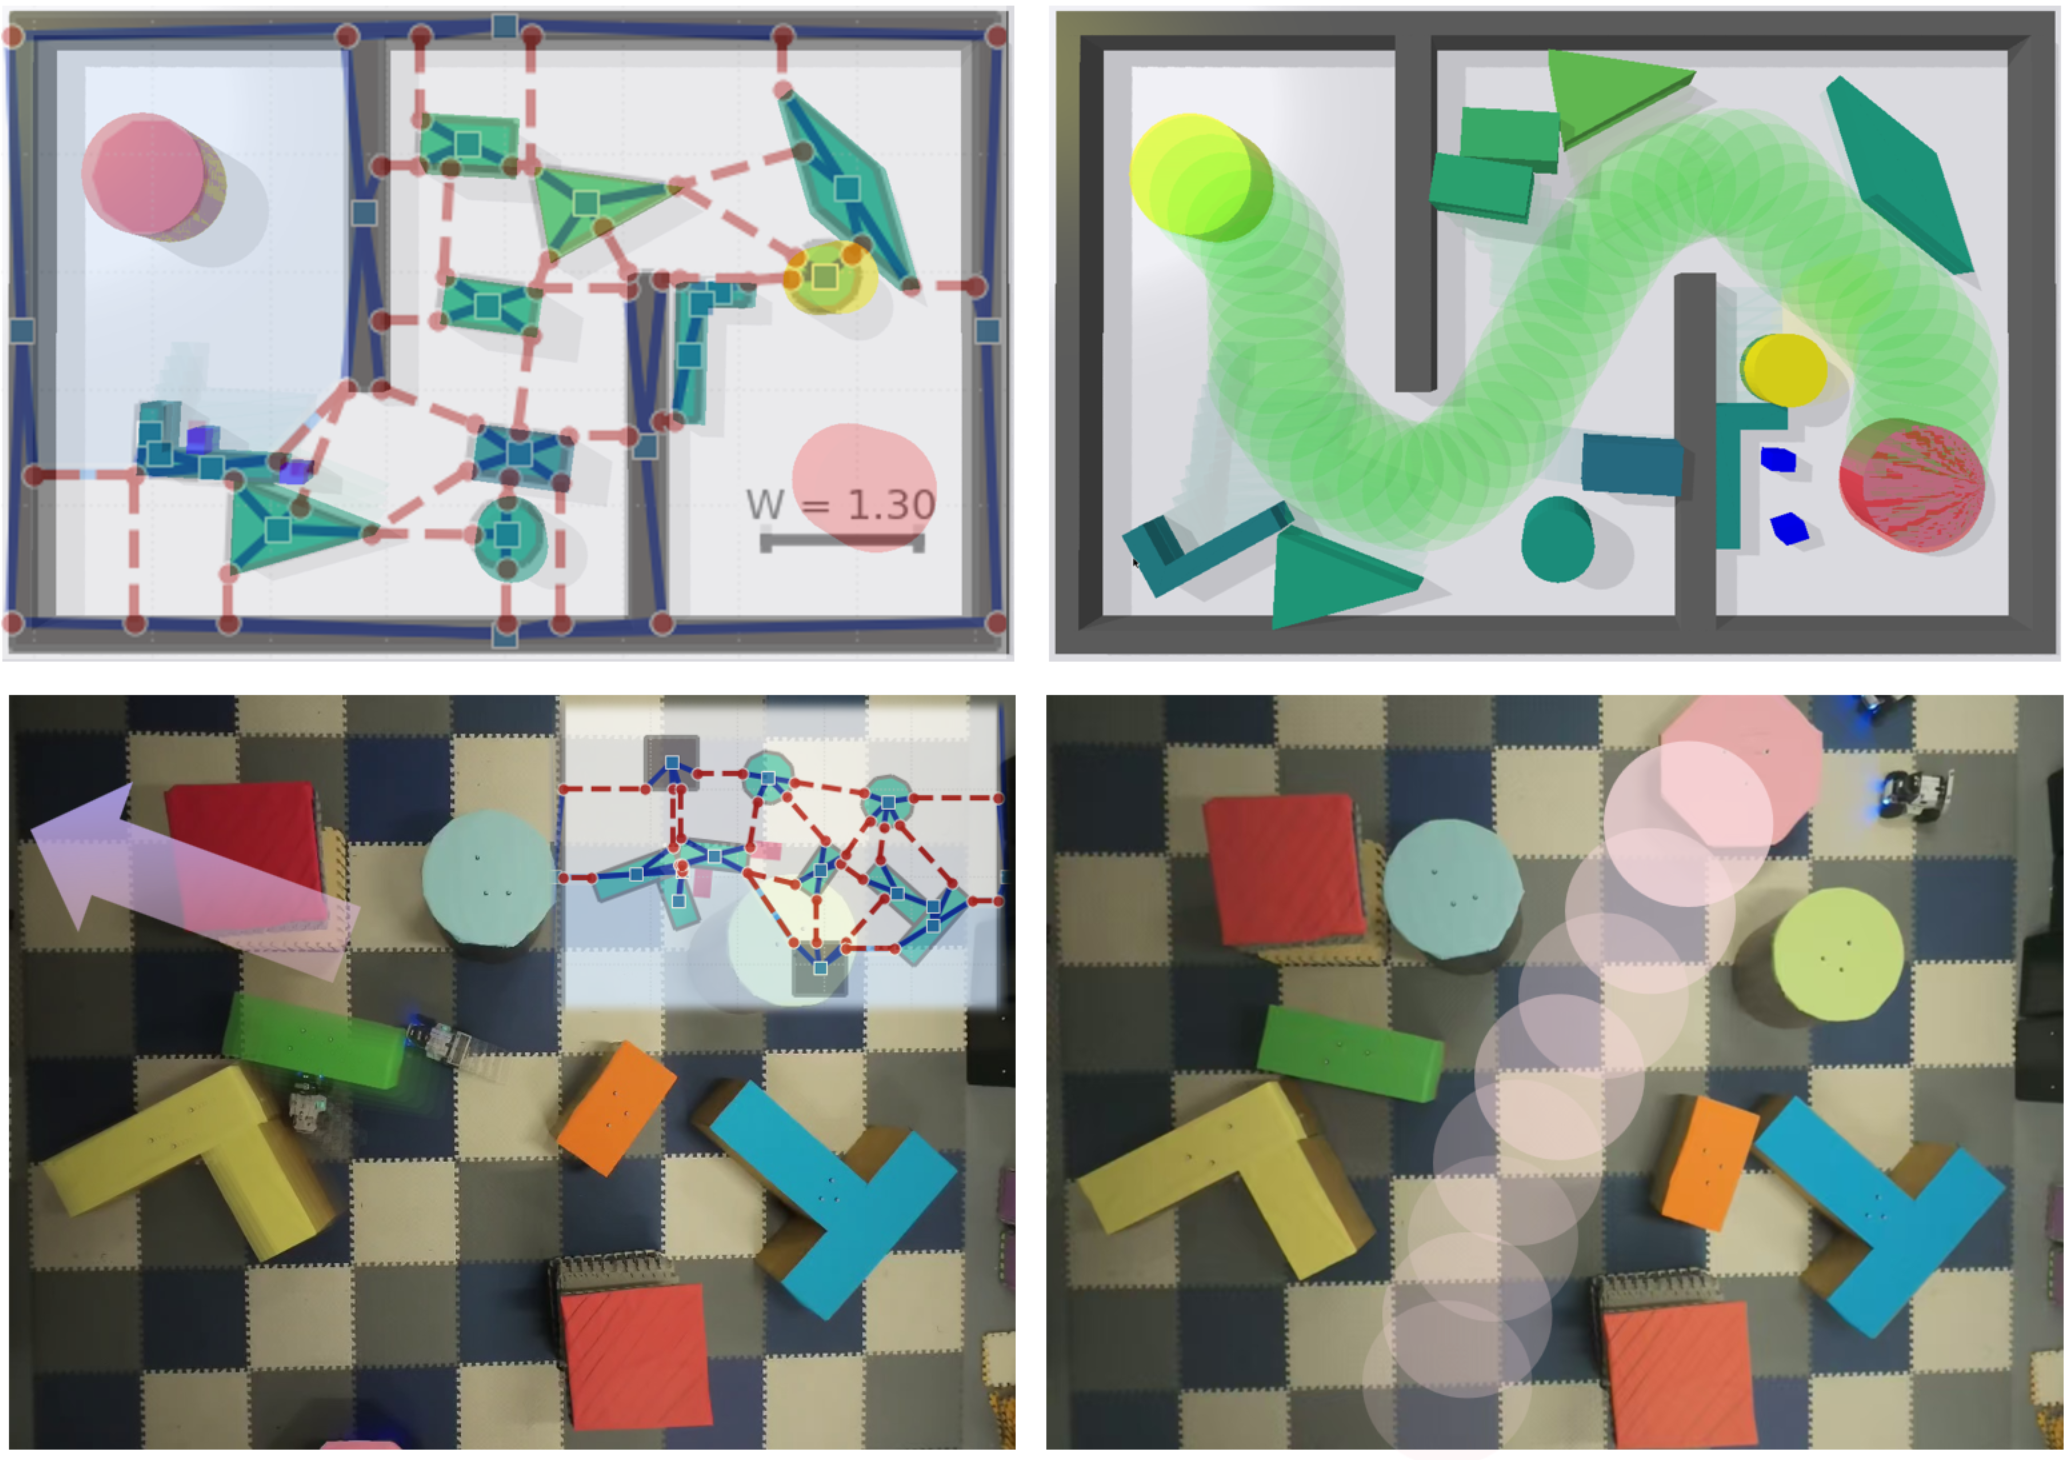
\includegraphics[width=\linewidth]{figures/cover.png}% or {presearch.pdf}
  \caption{
  Snapshots of collaborative path clearing system in both simulation and
  hardware. A team of mobile robots actively reconfigures movable
  obstacles to create a $W$-clear path for a large vehicle
  to traverse from start to goal.
  }
  \label{fig:snapshots}
\end{figure}

\subsection{Related Work}\label{subsec:intro-related}

Navigation Among Movable Obstacles (NAMO) has been studied as an extension of
motion planning in cluttered environments. Classical methods planned explicit
sequences of obstacle displacements through pushing, pulling, or
rotating~\cite{stilman2005navigation,stilman2007manipulation}, while later work
introduced heuristic search for scalability~\cite{stilman2007manipulation} and
graph- and sampling-based formulations for larger workspaces~\cite{yao2024local}.
Recent efforts extend NAMO to multi-agent settings where teams of robots clear
passages collaboratively~\cite{tang2024collaborative,ren2025search}. However,
most NAMO approaches still idealize robots as point agents with unlimited
actuation and neglect robot size, obstacle mass, and realistic dynamics, which
leads to plans that are geometrically valid but physically unrealizable.


%==============================================
\begin{figure*}[t!]
  \centering
  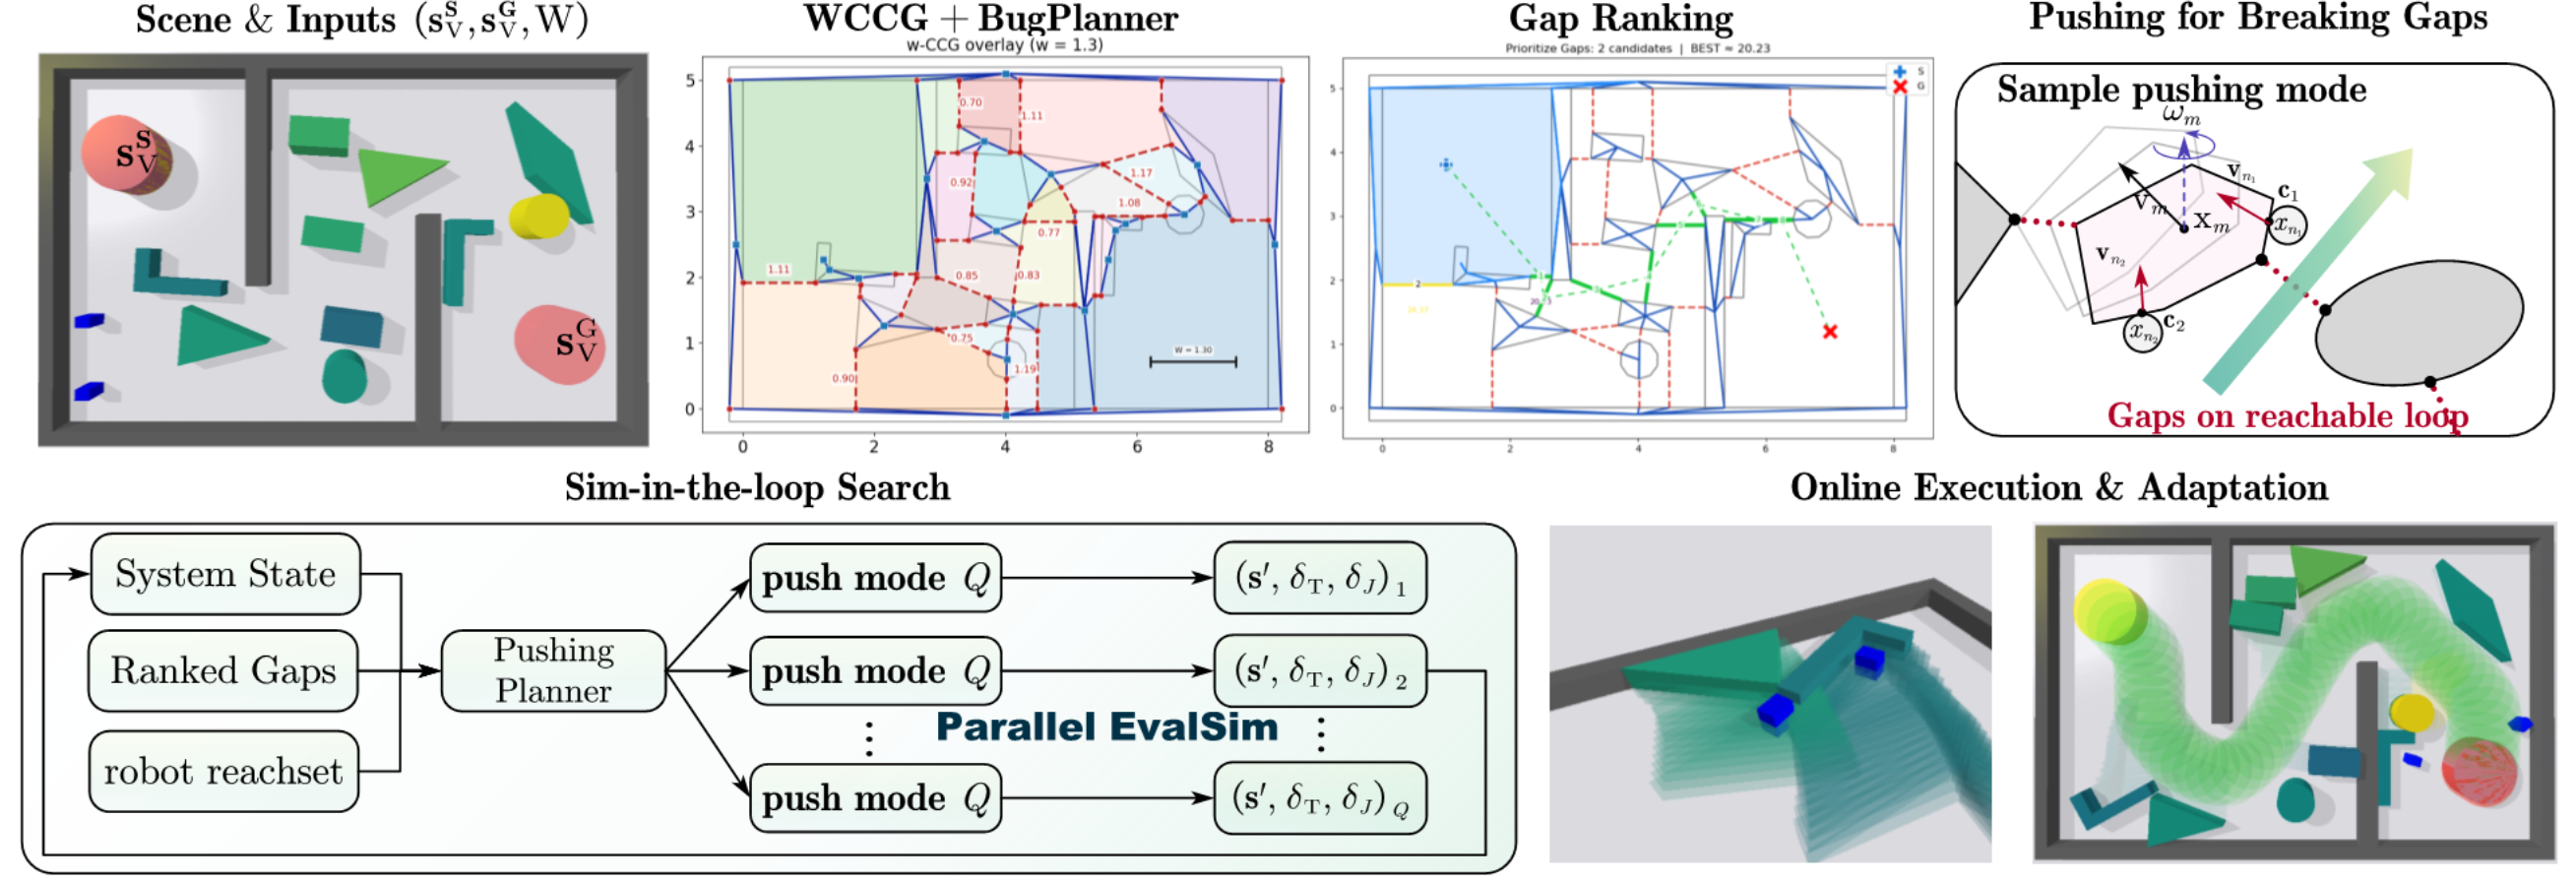
\includegraphics[width=\linewidth]{figures/overall.png}
  \vspace{-0.2in}
  \caption{Illustration of the W--Clearance Connectivity Graph (WCCG).
\textbf{Left:} Cluttered PyBullet scenario with the immovable walls and movable objects;
\textbf{Middle:} WCCG overlay with the centroid nodes (blue squares), bridge nodes
(red circles), centroid--bridge edges (blue), and bridge--bridge edges (red dashed)
annotated by the gap widths;
\textbf{Right:} Induced faces of the WCCG, where the colors indicate distinct connected
regions.}
  \label{fig:wccg}
  \vspace{-0.2in}
\end{figure*}
%==============================================


Collaborative pushing has also been widely investigated in multi-robot
manipulation. Foundational studies examined the mechanics of pushing and the
limit surface model~\cite{goyal1989limit,lynch1992manipulation}, while more
recent work addressed force synchronization~\cite{ni2023progressive}, contact
stability and slip margins~\cite{liu2025physics,chen2015occlusion}, and
cooperative transport of large payloads in structured
environments~\cite{ni2024physics,wang2006multi}. Learning-based approaches have
further explored emergent coordination in cluttered
settings~\cite{feng2025learning}. These studies demonstrate effective
multi-robot cooperation but are generally limited to single-object tasks and
assume strict collision avoidance with surrounding obstacles. As a result,
inter-object interactions and the coupled dynamics of multiple movable
obstacles remain largely unaddressed.

Physics-informed planning has emerged to integrate realistic dynamics into
motion generation. Several methods use physics engines to validate candidate
manipulations~\cite{lin2019efficient} or embed contact simulation directly in
the planning loop~\cite{rouxel2024multi}. Other approaches incorporate dynamic
models into planning for non-prehensile manipulation~\cite{zhou2017pushing,hou2020physics}
or apply learning with physics priors and differentiable physics for
contact-rich tasks~\cite{agrawal2016learning,ha2018reinforcement,ni2023progressive,liu2025physics}.
While these approaches highlight the benefits of embedding physical reasoning,
they often decouple high-level planning from low-level feasibility checks or
remain confined to single-object manipulation. Consequently, they do not scale
to collaborative path clearing in cluttered environments with many movable
obstacles.


%==============================
\subsection{Our Method}\label{subsec:intro-our}
This work introduces \emph{PushAround}, a physics-informed framework for
collaborative multi-robot pushing that actively constructs traversable
corridors for large vehicles in cluttered environments. The central novelty is
a hybrid search that jointly determines which obstacles to displace and how to
push them, coupling the high-level sequence of obstacle-clearing actions with
low-level pushing modes that specify contact points, directions, and forces.
The framework integrates three components: a W--Clearance Connectivity Graph
(WCCG) that certifies vehicle passage under width constraints, a gap-ranking
strategy that prioritizes frontier gaps by estimated effort, and a search
procedure that incrementally expands candidate plans while validating their
physical realizability. This integration guarantees that the resulting plans
are not only geometrically valid but also feasible under robot dimensions,
object mass, contact geometry, and coupled pushing dynamics. Efficiency is
achieved by combining compact geometric reasoning with prioritized evaluation,
focusing computation on the most promising actions and avoiding the scalability
issues of simulation-heavy NAMO approaches.

The contributions of this work are twofold: {(I)} it introduces the
first unified framework that couples multi-robot collaborative pushing with
physics-informed feasibility guarantees, producing executable plans for
path clearing in dense cluttered environments; and {(II)} it
demonstrates significant improvements in feasibility, efficiency, and
scalability over existing NAMO and collaborative pushing methods, through
extensive simulation and hardware validation.
